\section{304 --- Range Sum Query 2D - Immutable}
Given a 2D matrix matrix $M$, find the sum of the elements inside the rectangle defined by its upper left corner $(r_1, c_1)$ and lower right corner $(r_2, c_2)$.
\begin{figure}[H]
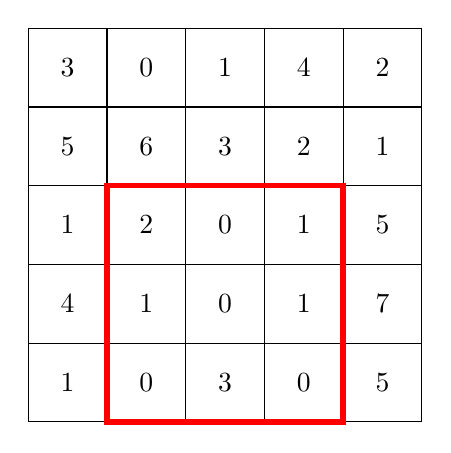
\begin{tikzpicture}
\draw[black, thin] (0,0) grid (5,5);
\node at (0.5,4.5) {$3$};
\node at (1.5,4.5) {$0$};
\node at (2.5,4.5) {$1$};
\node at (3.5,4.5) {$4$};
\node at (4.5,4.5) {$2$};
%row2
\node at (0.5,3.5) {$5$};
\node at (1.5,3.5) {$6$};
\node at (2.5,3.5) {$3$};
\node at (3.5,3.5) {$2$};
\node at (4.5,3.5) {$1$};
%row3
\node at (0.5,2.5) {$1$};
\node at (1.5,2.5) {$2$};
\node at (2.5,2.5) {$0$};
\node at (3.5,2.5) {$1$};
\node at (4.5,2.5) {$5$};
%row 4
\node at (0.5,1.5) {$4$};
\node at (1.5,1.5) {$1$};
\node at (2.5,1.5) {$0$};
\node at (3.5,1.5) {$1$};
\node at (4.5,1.5) {$7$};
%row 5
\node at (0.5,0.5) {$1$};
\node at (1.5,0.5) {$0$};
\node at (2.5,0.5) {$3$};
\node at (3.5,0.5) {$0$};
\node at (4.5,0.5) {$5$};
\draw[line width=2pt,red] (1,0) rectangle ++(3,3);
\end{tikzpicture}
\end{figure}
The above rectangle (with the red border) is defined by $(r_1, c_1) = (2, 1)$ and $(r_2, c_2) = (4, 3)$, which contains sum = 8.
\paragraph{Example:}
\begin{flushleft}
Give matrix $M$ is
\begin{table}[H]
    \begin{tabular}{ccccc}
        3 & 0 & 1 & 4 & 2 \\
        5 &  6 &  3 &  2 &  1\\
        1 &  2 &  0 &  1 &  5 \\
        4 &  1 &  0 &  1 &  7\\
        1 &  0 &  3 &  0 &  5
    \end{tabular}
\end{table}
\begin{lstlisting}[style=customc]
sumRegion(2, 1, 4, 3) // 8
sumRegion(1, 1, 2, 2) // 11
sumRegion(1, 2, 2, 4) // 12
\end{lstlisting}
\end{flushleft}
\paragraph{Note:}
\begin{itemize}
    \item You may assume that the matrix does not change.
    \item There are many calls to \texttt{sumRegion} function.
    \item You may assume that $r_1 \leq r_2$ and $c_1 \leq c_2$.
\end{itemize}
\subsection{Caching}
\begin{itemize}
    \item 这种方法类似于prefix sum的方式,这时候cumulative sum是相对于$(0,0)$的。
\end{itemize}
如下图所示,如果需要计算ABCD部分的sum $S$。将$S$用以$O$为原点的cumulative sum来表示。
\definecolor{lightblue}{RGB}{229,241,255}
\begin{enumerate}
\item Cumulative sum from $O$ to $D$, denote as $S_0$
\begin{figure}[H]
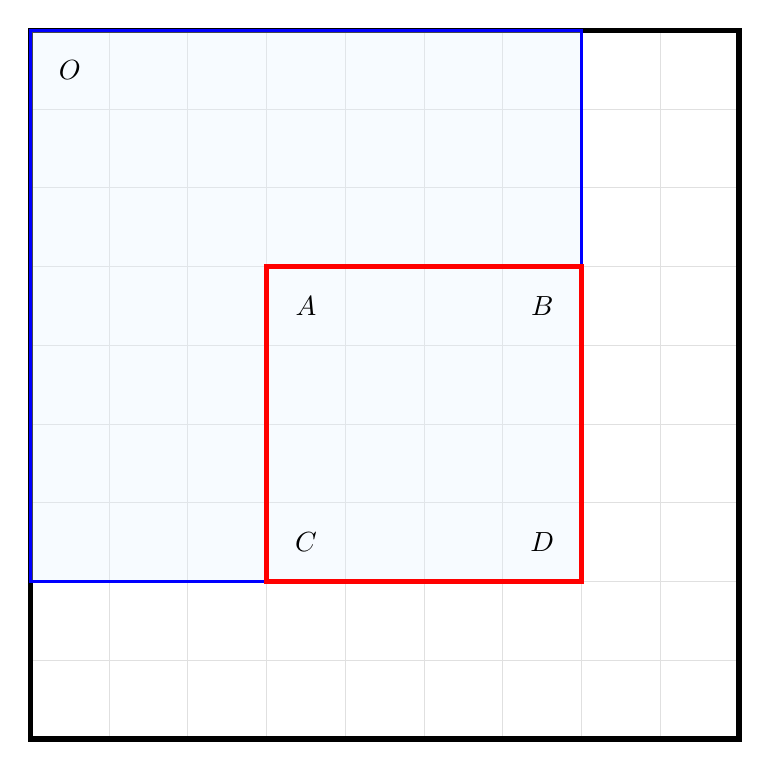
\begin{tikzpicture}
\draw[thin,color=white!60!black!30] (0,0) grid (9,9);
\draw[line width=2pt, color=black] (0,0) rectangle (9,9);
\draw[line width=1pt, color=blue, fill=lightblue, fill opacity=0.3] (0,9) rectangle ++(7,-7);
\node at (0.5,8.5) {$O$};
\node at (3.5,2.5) {$C$};
\node at (3.5,5.5) {$A$};
\node at (6.5,2.5) {$D$};
\node at (6.5,5.5) {$B$};
\draw[line width=2pt, color=red] (3,2) rectangle (7,6);
\end{tikzpicture}
\end{figure}
    \item Cumulative sum from $O$ to the top of $B$, denote as $S_1$
\begin{figure}[H]
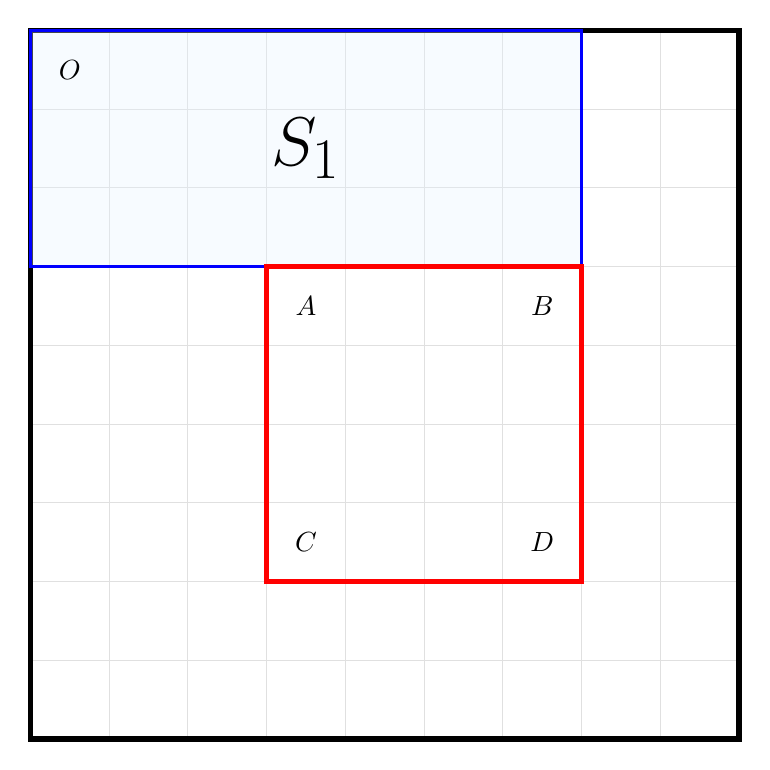
\begin{tikzpicture}
\draw[thin,color=white!60!black!30] (0,0) grid (9,9);
\draw[line width=2pt, color=black] (0,0) rectangle (9,9);
\draw[line width=1pt, color=blue, fill=lightblue, fill opacity=0.3] (0,9) rectangle ++(7,-3);
\node at (0.5,8.5) {$O$};
\node at (3.5,2.5) {$C$};
\node at (3.5,5.5) {$A$};
\node at (6.5,2.5) {$D$};
\node at (6.5,5.5) {$B$};
\node at (3.5,7.5) [minimum size=2cm] {\Huge $S_1$};
\draw[line width=2pt, color=red] (3,2) rectangle (7,6);
\end{tikzpicture}
\end{figure}
\item Cumulative sum from $O$ to the left of $C$, denote as $S_2$
\begin{figure}[H]
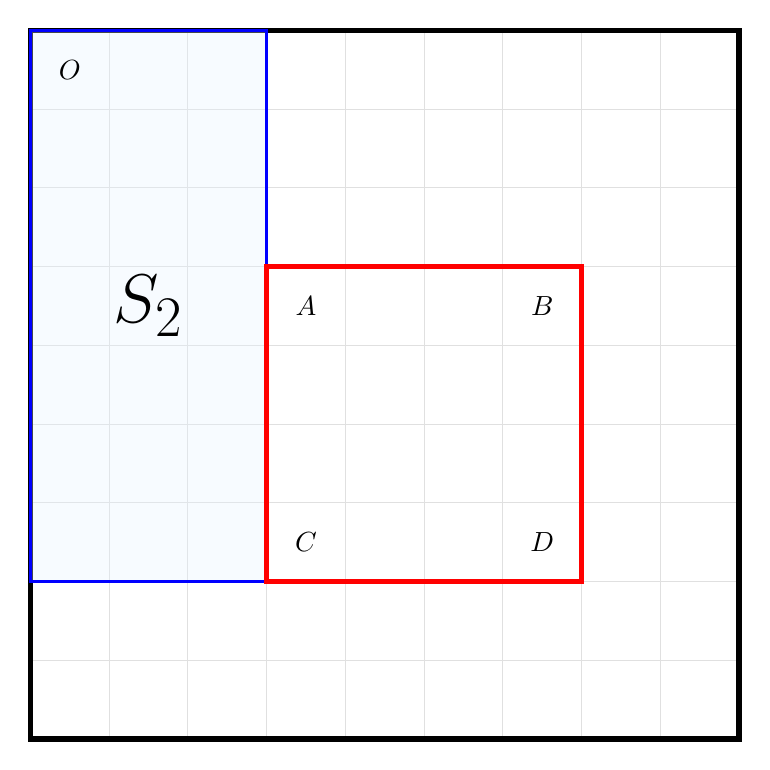
\begin{tikzpicture}
\draw[thin,color=white!60!black!30] (0,0) grid (9,9);
\draw[line width=2pt, color=black] (0,0) rectangle (9,9);
\draw[line width=1pt, color=blue, fill=lightblue, fill opacity=0.3] (0,9) rectangle ++(3,-7);
\node at (0.5,8.5) {$O$};
\node at (3.5,2.5) {$C$};
\node at (3.5,5.5) {$A$};
\node at (6.5,2.5) {$D$};
\node at (6.5,5.5) {$B$};
\node at (1.5,5.5) [minimum size=2cm] {\Huge $S_2$};
\draw[line width=2pt, color=red] (3,2) rectangle (7,6);
\end{tikzpicture}
\end{figure}
\item Cumulative sum from $O$ to top left of $A$, denote as $S_3$
\begin{figure}[H]
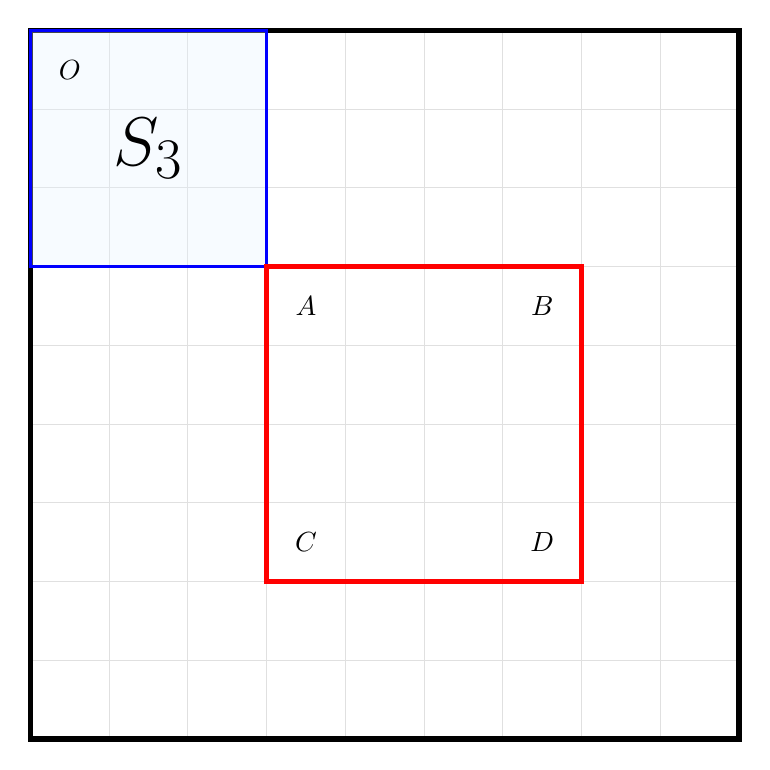
\begin{tikzpicture}
\draw[thin,color=white!60!black!30] (0,0) grid (9,9);
\draw[line width=2pt, color=black] (0,0) rectangle (9,9);
\draw[line width=1pt, color=blue, fill=lightblue, fill opacity=0.3] (0,9) rectangle ++(3,-3);
\node at (0.5,8.5) {$O$};
\node at (3.5,2.5) {$C$};
\node at (3.5,5.5) {$A$};
\node at (6.5,2.5) {$D$};
\node at (6.5,5.5) {$B$};
\node at (1.5,7.5) [minimum size=2cm] {\Huge $S_3$};
\draw[line width=2pt, color=red] (3,2) rectangle (7,6);
\end{tikzpicture}
\end{figure}
\item 注意到$S_1$和$S_2$都包括了$S_3$,因此$S=S_0-S_1-S_2+S_3$
\item 用一个二维数组$F$来记录从$O$到当前坐标$(r,c)$的cumulative sum,注意到$F$的dimension类似于一维的prefix sum,如果matrix的dimension是$m\times n$,那么F的dimension就是$(m+1)\times(n+1)$。因此在坐标$(r,c)$的$F$其实是$F[r+1][c+1]$。于是有$F[r+1][c+1]=F[r+1][c]+F[r][c+1]+M[r][c]-F[r][c]$。因为都$F[r+1][c]$和$F[r][c+1]$都
包括了$F[r][c]$。
\item 对于从$(r_1,c_1)$到$(r_2,c_2)$的sum $S$,用$F$来表示,即为$S=F[r_2+1][c_2+1] - F[r_1][c_2+1] - F[r_2+1][c_1] + F[r_1][c_1]$。其中$F[r_2+1][c_2+1]$, $F[r_1][c_2+1]$,$F[r_2+1][c_1]$和$F[r_1][c_1]$分别为上述分析中的$S_0$,$S_1$,$S_2$和$S_3$
\end{enumerate}
\setcounter{lstlisting}{0}
\begin{lstlisting}[style=customc, caption={Caching}]
class NumMatrix {
public:
    NumMatrix(vector<vector<int>> matrix) {
        
        if(matrix.empty() || matrix[0].empty())
        {
            s=matrix;
            return;
        }
        
        vector<vector<int>> tmp(matrix.size()+1, vector<int>(matrix[0].size()+1,0));
        s.swap(tmp);
        
        for(size_t i = 0; i< matrix.size(); ++i)
        {
            for(size_t j = 0; j < matrix[0].size(); ++j)
            {
                s[i+1][j+1] = s[i+1][j] + s[i][j+1] + matrix[i][j] - s[i][j];
            }
        }
    }
    
    int sumRegion(int row1, int col1, int row2, int col2) {
        if(s.empty() || s[0].empty())
        {
            return 0;
        }
        
        return s[row2+1][col2+1] - s[row1][col2+1] - s[row2+1][col1] + s[row1][col1];
    }
    
    vector<vector<int>> s;
};
\end{lstlisting}

\paragraph{Related Problems}
\begin{itemize}
\item \textbf{303. Range Sum Query - Immutable}
\item \textbf{308. Range Sum Query 2D - Mutable}
\end{itemize}